\chapter{Analysis and Discussion}
\label{sec:aus}

In the following, the experimental findings are presented and subsequently discussed.
To begin with, \autoref{sec:SN} determines the noise of the setup and examines its dependence
on the time constant of the lock-in amplifier.
As a further preparatory step, the size of the beam is determined using the cutting-knife
method, and the resulting values are then used to calculate the power per unit area.
Subsequently, \autoref{sec:AZnTe} examines and establishes the baseline values for the quality
of the THz radiation by evaluating the transients and their Fourier transforms.
For this, the behavior of the amplitude at different laser powers is analyzed.
These steps are then repeated for the two organic crystals OH1 and BNA in \autoref{sec:AOH1}
and \autoref{sec:ABNA} and compared with the known values from \autoref{sec:AZnTe}.


\section{Determination of the Noise Floor}
\label{sec:SN}
The noise is measured under various conditions, distinguishing between mains-powered and
battery-powered supply.
This distinction is made in order to separate interference sources such as ground loops and
mains hum from the intrinsic electronic noise.
For the mains supply, the noise is measured both with the laser switched on and with it
switched off. \\



% To check the noise, only the probe beam is let through the setup and the pump beam is
% blocked.
% As a result, no change in polarization occurs in the detection crystal, and the two
% components generated by the Wollaston prism are identical.
% Thus the measured signal should theoretically be 0.
% For this, it was also carried out completely without illumination by the laser, in order
% to see the difference between the noise caused only by the setup and the noise added by
% the laser itself, since it also does not function perfectly.


\autoref{fig:tc1} shows the values for the measurements with mains supply, with the laser
switched on and switched off, respectively.
In the case with the laser switched on, however, only the detection beam is let through while
the pump beam is blocked, so that only the noise is measured here as well.
The time constant $\tau$ is then varied from $\SIrange{30}{3000}{\milli\second}$ on the
lock-in amplifier.
At each time constant, a measurement was taken for $\SI{20}{s}$, and the mean value was then
determined.

\begin{figure}
    \centering
    \begin{subfigure}[b]{0.48\textwidth}
        \centering
        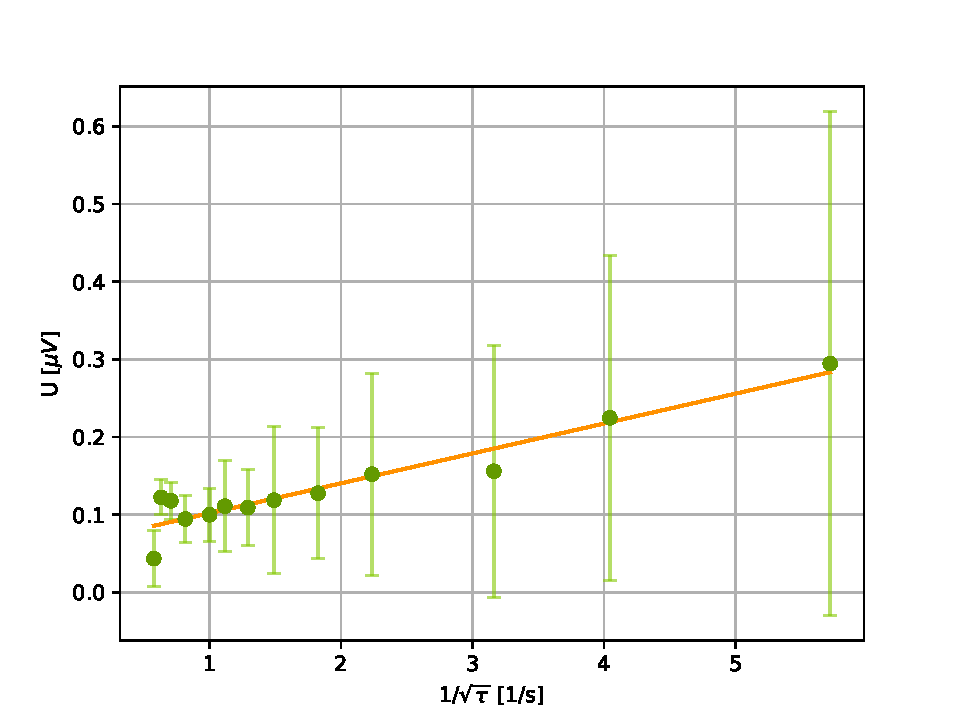
\includegraphics[width=\textwidth]{content/plots/pdf/time_constant/time_constant_oi.pdf}
        \caption{Without illumination.}
        \label{fig:tco}
    \end{subfigure}
    \hfill
    \begin{subfigure}[b]{0.48\textwidth}
        \centering
        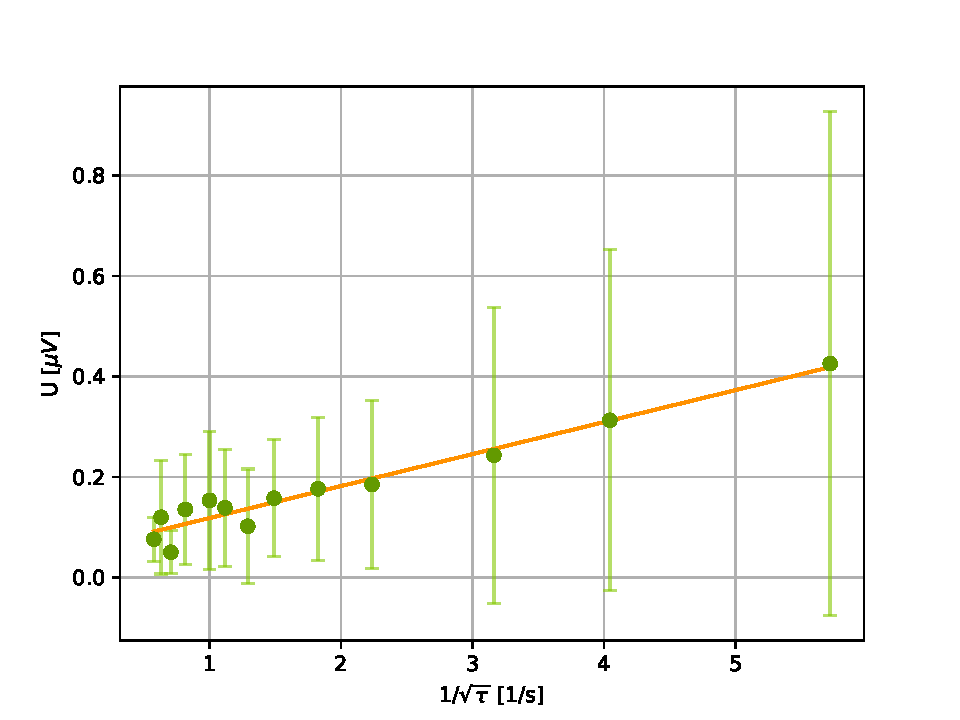
\includegraphics[width=\textwidth]{content/plots/pdf/time_constant/time_constant_wi.pdf}
        \caption{With illumination.}
        \label{fig:tcw}
    \end{subfigure}
    \caption{Measured values of the noise voltage plotted against $\frac{1}{\sqrt{\tau}}$. Also
    shown is a fit of the form $\frac{A}{\sqrt{\tau}}+b$.}
    \label{fig:tc1}
\end{figure}

The resulting values are shown in \autoref{fig:tc1}, with \autoref{fig:tco} showing the data
without illumination by the laser and \autoref{fig:tcw} with illumination.
For both, a fit of the form \autoref{eqn:tc} was performed, where $A$ is the noise amplitude
of the measurement and $b$ is the offset of the noise floor.
The fit gives the values
\begin{align}
    \label{tab:tc1}
    A_\text{mi} =&\SI{6.4+-0.5e-8}{\volt} & b_\text{mi} =&\SI{5.5+-1.1e-8}{\volt} \\
    A_\text{oi} =&\SI{3.9+-0.4e-8}{\volt} & b_\text{oi} =&\SI{6.3+-1e-8}{\volt}\, .
\end{align}
It is found that the noise amplitude with illumination is approximately a factor of 2 larger
than without illumination.
This factor can be explained by the fact that shot noise is added at the photodiodes when
light is incident on them.
This arises from the statistical process of the photoelectric effect, which generates the
current at the photodiode.
This only occurs when a single photon has enough energy to raise an electron to a higher
shell; since the energy of the photon is statistically distributed, this introduces an
uncertainty into the measurement.
However, this uncertainty averages out over long time constants.
This is clearly visible, since at higher time constants the two converge to a similar
offset $b$.\\
Furthermore, this measurement was repeated, but with the power supply of the photodiodes
provided not by power generators operated from the mains, but by batteries.
To cover a further aspect here, averaging was carried out once over $\SI{20}{\second}$ and
once over $\SI{60}{\second}$.
The resulting values are shown in \autoref{fig:tc2}.
Here, \autoref{fig:tc20} is the plot for a measurement duration of \SI{20}{\second}, and
\autoref{fig:tc60} the plot for \SI{60}{\second}.
A fit is then created using \autoref{eqn:tc}.
Here, for both data series, the value with the lowest time constant
($\tau= \SI{30}{\milli\second}$) is not taken into account, since due to its very large error
no statement can be made about its relative position to the other values.



\begin{figure}
    \centering
    \begin{subfigure}[b]{0.48\textwidth}
        \centering
        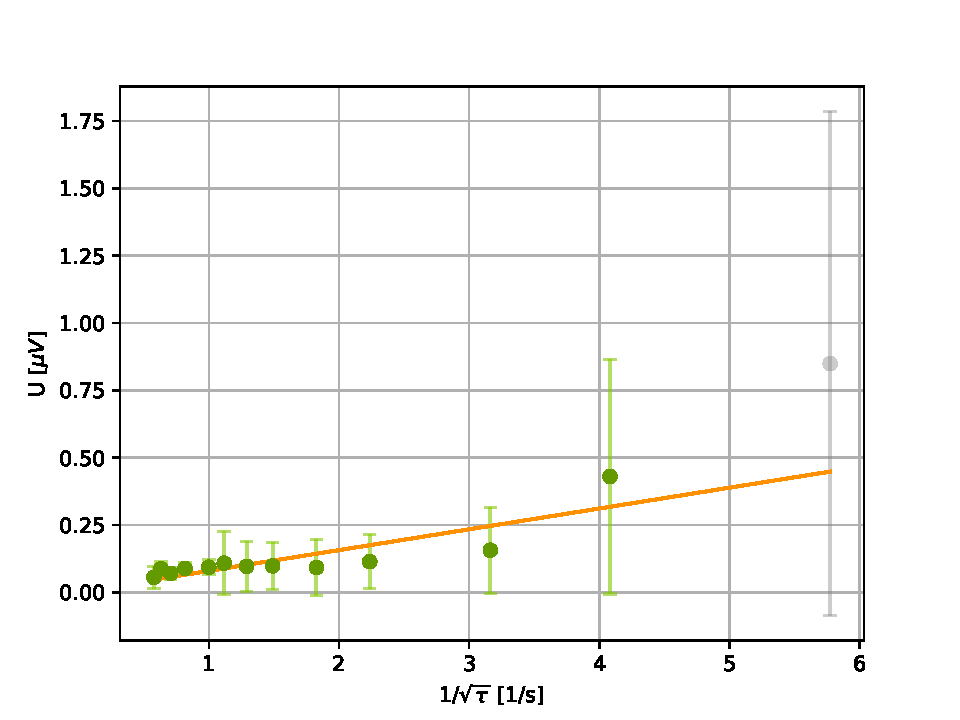
\includegraphics[width=\textwidth]{content/plots/pdf/time_constant/time_constant_b20.pdf}
        \caption{Measurement with a measurement interval of $\SI{20}{\second}$.}
        \label{fig:tc20}
    \end{subfigure}
    \hfill
    \begin{subfigure}[b]{0.48\textwidth}
        \centering
        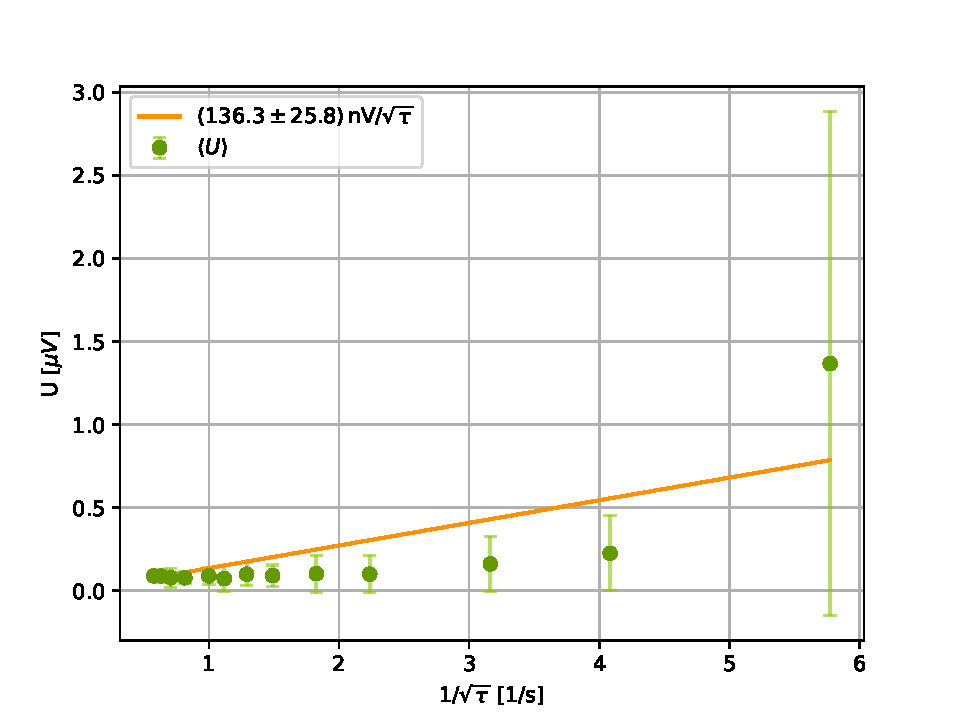
\includegraphics[width=\textwidth]{content/plots/pdf/time_constant/time_constant_b60.pdf}
        \caption{Measurement with a measurement interval of $\SI{60}{\second}$.}
        \label{fig:tc60}
    \end{subfigure}
    \caption{Measured values of the noise voltage with battery-powered supply and no
        illumination by the laser. Also shown is a fit through the measured values of the
        form $\frac{A}{\sqrt{\tau}}+b$.}
    \label{fig:tc2}
\end{figure}

The values resulting from the fit are shown in \autoref{tab:tc2}.

\begin{align}
    \label{tab:tc2}
    A_\text{20\,s} =&\SI{7.7+-1.5e-08}{\volt} & b_\text{20\,s} =&\SI{0.28+-2.9e-08}{\volt} \\
    A_\text{60\,s} =&\SI{3.7+-0.47e-08}{\volt} & b_\text{60\,s} =&\SI{4.8+-0.9e-08}{\volt}\, .
\end{align}

The values show that the noise amplitude with batteries is worse or comparable, as can be
seen in \autoref{tab:tc1}.
The offset $b$, on the other hand, is lower, but is subject to such a large error that no
statement can be made about it.
In addition, the noise amplitude $A$ for the longer measurement time is about half as large
as for the short measurement time.
The offset, however, is one order of magnitude larger than that of the measurement with
$\SI{20}{\second}$, whereby the value $b_{\text{60\,s}}$ has no real significance.

All the measurement data are summarized in \autoref{fig:tcc}.
These show that the noise decreases with increasing time constant $\tau$ and reaches a
plateau from $\tau=\SI{0.3}{\second}$ onward, at which the noise changes only minimally.
However, it is already apparent at the beginning that the noise with the laser switched on
and low time constants is significantly higher than with the laser switched off.
This can be explained by the shot noise.
\begin{figure}
    \centering
    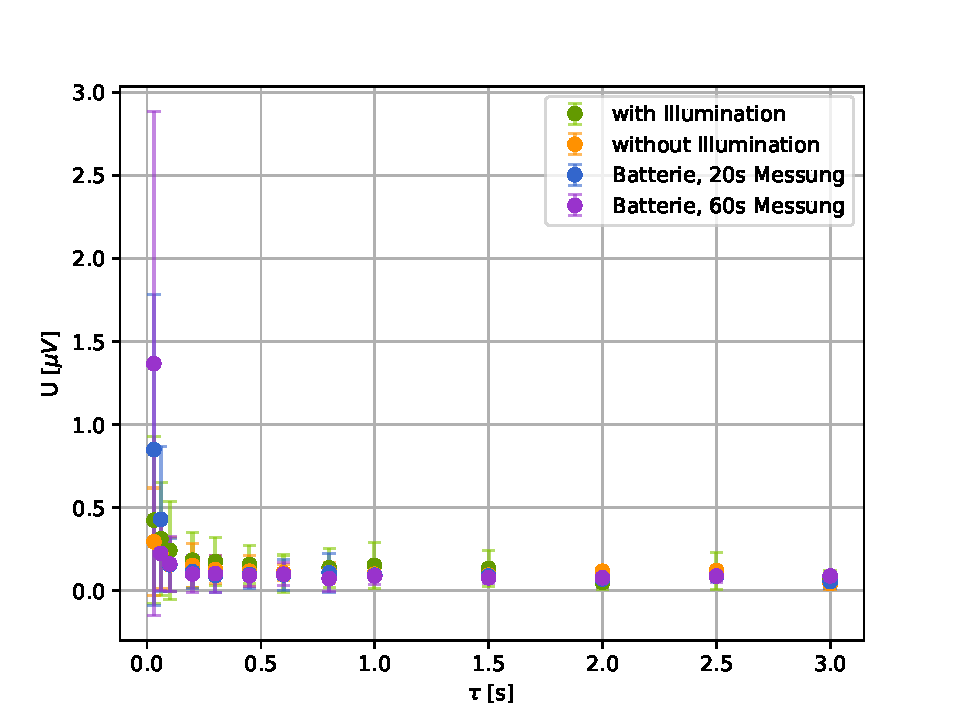
\includegraphics[width=0.8\textwidth]{content/plots/pdf/time_constant/time_constant_combined_vs_tau.pdf}
    \caption{Comparison of the noise voltage with and without the laser switched on.
    Also shown are the values with the battery as power supply for different averaging
    times.}
    \label{fig:tcc}
\end{figure}
This statistical process can, however, be averaged out by a longer time constant, which is
why the noise decreases at higher time constants.
The offset $b$, i.e. the background noise, can be explained by the electronic noise in the
detection components.
Since the same detection components are used for all measurements, this noise is also
always similar.
As described above, it can be seen that from a time constant of $\tau=\SI{0.3}{\second}$
onward, no major improvement is observed.
Therefore, this bachelor's thesis works with a time constant of $\tau=\SI{0.1}{\second}$, but
with 5 measurements taken at the same position, which means that the time constant
effectively increases to $\SI{0.5}{\second}$.
This approach was chosen to speed up the measurement process, since the measurement program
waits several time constants before each individual measurement before it measures.
The shorter individual time constant reduces this waiting time, while the quality of the
measurement data is preserved by the subsequent averaging over 5 measurements.


% This can be explained by the fact that the laser triggers statistical processes such as
% shot noise, thereby introducing a further uncertainty into the measurement.
% The offset value $b$ is nearly identical and lies within the error.
% Thus it can be assumed that the baseline noise depends only on the electronics and not on
% the laser beam.

% For this, a comparison of the two data series can be seen in \autoref{fig:tcc}.
% There it can be seen that at the beginning the difference is still clearly visible, but
% becomes smaller with increasing time constant and can no longer be reliably determined
% from a time constant of about $0.8\,\unit{s}$ onward.
% This means that for the remaining measurements, a time constant of at least
% $0.8\,\unit{s}$ should be chosen.
% show that for the following measurement a time constant $\tau \ge 0.8\,\unit{s}$ is
% sensible, so that the noise, e.g. from shot noise, is averaged out and a measurement as
% free of noise as possible can be performed.

%--------------------------------------------Abschnitt Spot größe
\section{Spot Size}
\label{sec:spot}
Since the organic crystals are extremely small while the laser beam is significantly larger,
the size of the laser beam is determined in the following, which can then be used to
determine the power density.
These values serve as a reference in the following chapters for the power acting on the
crystals. \\
The knife-edge method is used to determine the beam size.
This is based on mounting a razor blade on an adjustable platform and holding it into the
beam.
This setup is placed at the position where the generation crystals are also placed.
The power is measured behind this position.
To determine the beam size, the razor blade is then moved in steps of $\SI{0.05}{\milli\meter}$,
so that more of the beam is blocked by the blade and the measured power decreases
accordingly.
For each adjustment, the difference in power between two consecutive measured values is
determined.
This difference approximately corresponds to the power falling on the area additionally cut
off in this step.
This difference was determined once each in the x- and y-directions.
The corresponding measurement data are shown in \autoref{fig:spot_c}.

\begin{figure}
    \centering
    \begin{subfigure}[b]{0.48\textwidth}
        \centering
        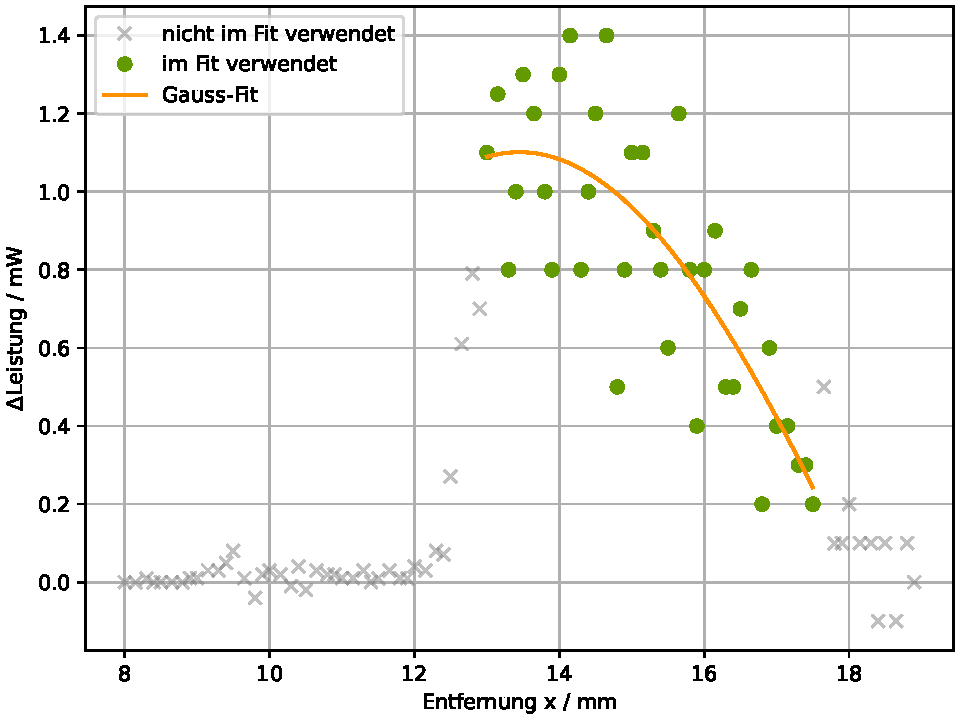
\includegraphics[width=0.8\textwidth]{content/plots/pdf/spot_size_x.pdf}
        \caption{Difference between the measured values of two consecutive power readings
        in the x-direction.
        }
        \label{fig:spot_x}
    \end{subfigure}
    \hfill
    \begin{subfigure}[b]{0.48\textwidth}
        \centering
        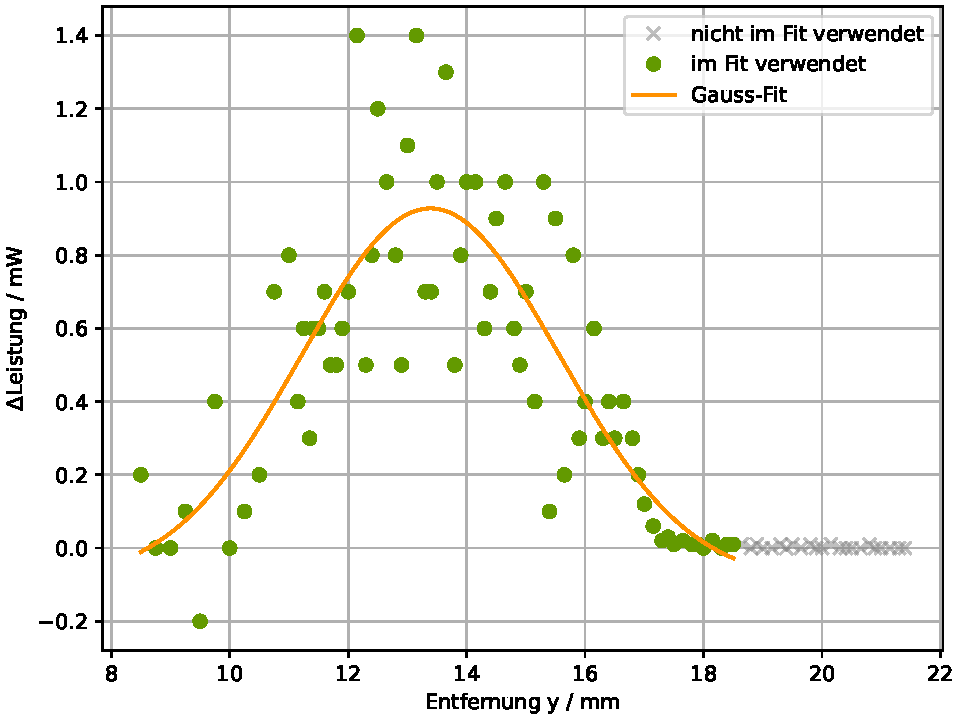
\includegraphics[width=0.8\textwidth]{content/plots/pdf/spot_size_y.pdf}
        \caption{Difference between the measured values of two consecutive power readings
        in the y-direction.}
        \label{fig:spot_y}
    \end{subfigure}
    \caption{Differences in power as the razor blade is moved along different axes.}
    \label{fig:spot_c}
\end{figure}


In \autoref{fig:spot_x}, a noticeably steeper drop can be seen on the left side than on the
right.
This suggests that the beam is being clipped by an optical component earlier in the beam
path, so this is not the ideal shape of the beam, and this side therefore cannot be used to
infer the actual size of the beam.
For this reason, only the right side is used for the x-direction to perform a Gaussian fit
of the form
\begin{equation}
    f(x) = A\cdot \exp\left(-\frac{1}{2}\left(\frac{x-\mu}{\sigma}\right)^2\right) + b
\end{equation}

.
For the y-direction, on the other hand, the fit could be determined using both sides.
Using the fit, the following coefficients are obtained
\begin{align}
    A_x &= \SI{1.246+-0.150}{mW} & \mu_x &= \SI{13.865+-0.214}{mm} \\
    \sigma_x &= \SI{2.452+-0.429}{mm} & b_x &= \SI{-0.141+-0.152}{mW} \\
    A_y &= \SI{1.021+-0.118}{mW} & \mu_y &= \SI{13.388+-0.126}{mm} \\
    \sigma_y &= \SI{2.178+-0.331}{mm} & b_y &= \SI{-0.093+-0.128}{mW} \,.
\end{align}
Using these values and $w=2\cdot\sigma $, the radius for the respective axes can be
determined.
This gives
\begin{align}
	w_x &= \SI{4.905+-0.858}{\milli\meter} \ \text{and}\\
	w_y &= \SI{4.356+-0.662}{\milli\meter} \, .
\end{align}
It is found that the x-size is larger, which can be attributed to the fit being performed on
only one side due to the clipped beam.
The beam is therefore elliptical, and $A = \pi w_x w_y$ is used for the area.
This gives an area of $\SI{67.1+-15.7}{\milli\meter\squared}$, where the large error results
from the fit in the x-direction.
The power of the beam at this position is $\SI{34.5}{\milli\watt}$.
From this, the peak intensity can be determined using $I_\text{sp}= \frac{2\cdot P}{A}$.
This gives $\SI{0.103+-0.024}{\watt\per\centi\meter\squared}$.
Here, the error of almost $24\,\%$ should be noted, this large deviation being explained by
the one-sided fit in the x-direction.
It should also be noted that this is the average peak intensity.
However, the laser is a pulsed laser, so the power of a single pulse is many times higher
than this averaged value.
As a reference value, however, this value is still useful, since all measurements were
taken with the same laser and are therefore comparable via this value.
This value per unit area is necessary because the OH1 and BNA samples do not fill the
entire beam, so the measured values would not be comparable to those of ZnTe, which does
fill the entire beam.
In the following, this baseline measurement with ZnTe is described.

\section{ZnTe}
\label{sec:AZnTe}
In order to have a comparison for the organic emitters, a measurement of the THz radiation
generated by ZnTe is carried out first.
In contrast to the other crystals, the entire power of the pump beam could be used for
generation, since the ZnTe crystal is large enough to fill the entire beam.
First, the position of "time zero", i.e. the position of the first and largest peak of the
THz pulse, is determined.
Subsequently, an interval from $\SI{-3}{ps}$ to $\SI{11}{ps}$ around this value was measured.
This transient for a pump power of $\SI{55}{mW}$ is shown in \autoref{fig:ZnTeT}.
In this, time zero is marked at 0, followed by the ringing that can be seen afterward.
Ringing occurs because the pulse does not exit the generation crystal in a straight line
while passing through it, and parts of the pulse exit the crystal at a later time via
multiple reflection.
As a result, a small part reaches the detection crystal only later and is therefore also
measured later, which can be seen as a second pulse at around $\SI{7}{ps}$.

\begin{figure}[H]
    \centering
    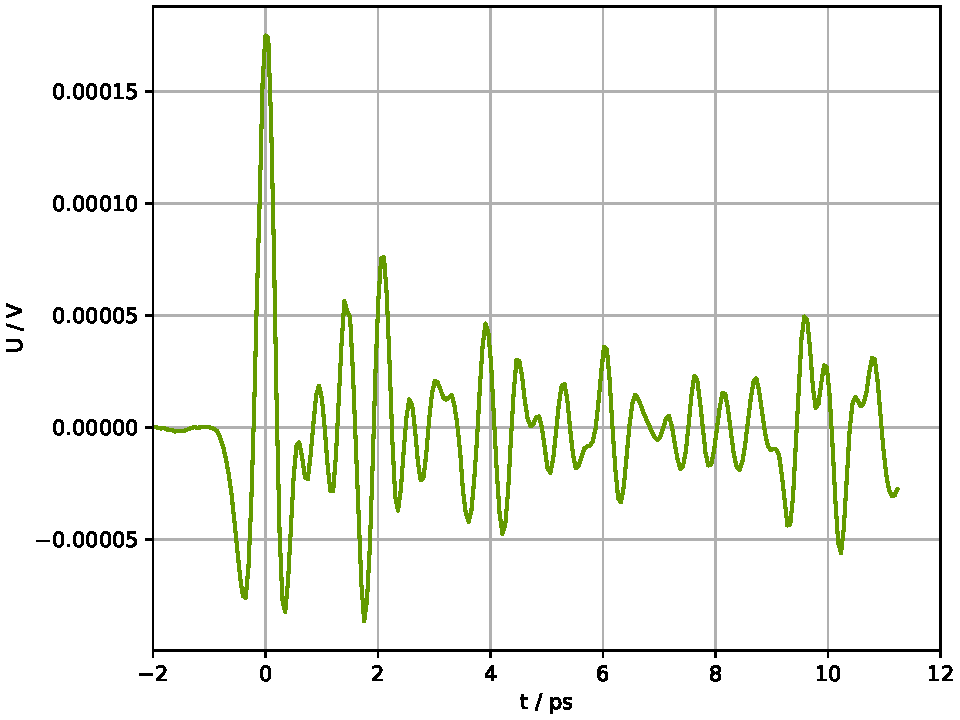
\includegraphics[width=0.8\textwidth]{content/plots/pdf/ZnTe/110mW.pdf}
    \caption{Transient of the THz pulse generated by ZnTe at a pump power of
    $\SI{55}{\milli\watt}$.}
    \label{fig:ZnTeT}
\end{figure}

This transient was measured for various pump powers, and the peak-to-peak values were
determined.
\autoref{fig:ampc} lists these values, together with a linear fit to show the linear
dependence on the laser power.
It should be noted that the power of $\SI{55}{mW}$ is not the highest possible power of the
laser, but from this power onward the crystal begins to become luminescent, which is a sign
of being close to the damage threshold.
To avoid damaging the crystal, the power was therefore not increased further.
The signal-to-noise ratio can also be determined from the transient and the peak-to-peak
values.
For this, the peak-to-peak value of the individual powers is divided by the noise value
determined in \autoref{sec:SN}.
The noise value for a time constant of $\tau = \SI{450}{\milli\second}$ and illumination,
which is $U_\text{Rauschen}=\SI{0.158}{\micro\volt}$, is used as a uniform noise reference
for all powers.
This value is used because it is the closest measured value to the theoretically used time
constant of $\tau=\SI{500}{ms}$.
The resulting values for the signal-to-noise ratio for the different powers are listed in
\autoref{tab:snZnTe}.
Notable here are the values between $\SI{30}{\milli\watt}$ and $\SI{48}{\milli\watt}$. Here,
a strong increase relative to the other values can be seen in the peak-to-peak value.
Between these and the other measurements, various voltage sources for the photodiodes were
tested; these did not turn out to be ideal, and the setup was switched back to the mains
supply.
It appears that the settings on the voltage sources were altered in the process, which could
explain the suddenly higher values of the measurement.

\begin{table}
    \centering
    \caption{Peak-to-peak amplitude and the resulting signal-to-noise ratio of the ZnTe
    transients at various pump powers, relative to the uniform noise reference
    $U_\text{Rausch}=\SI{0.158}{\micro\volt}$ at $\tau=\SI{450}{ms}$.}
    \label{tab:snZnTe}
    \begin{tabular}{S[table-format=3.0] S[table-format=3.1] S[table-format=4.1]}
        \toprule
        {$P \mathrel{/} \si{\milli\watt}$} & {$U_\text{ptp} \mathrel{/} \si{\micro\volt}$} & {SNR} \\
        \midrule
        2   & 15.4  & 97.3   \\
        3.3  & 18.7  & 118.5  \\
        7.4  & 46.9  & 296.6  \\
        8  & 77.5  & 490.7  \\
        13  & 88.8  & 561.9  \\
        18  & 116.2 & 735.3  \\
        24  & 143.7 & 909.2  \\
        30  & 261.3 & 1653.7 \\
        34  & 306.2 & 1938.0 \\
        40  & 353.8 & 2239.4 \\
        48  & 386.7 & 2447.7 \\
        55 & 261.4 & 1654.3 \\
        \bottomrule
    \end{tabular}
\end{table}



Furthermore, a Fourier transform is performed on the transients; this is shown for
$\SI{5}{mW}$ in \autoref{fig:ZnTeF}.
The Fourier transform shows which frequencies are present in the transient of the THz pulse.
From this, the bandwidth of the THz pulse can be determined.
This is $\SI{2.4}{\tera\hertz}$.
Frequencies between $\SI{0.2}{\tera\hertz}$ and $\SI{2.6}{\tera\hertz}$ are generated.
Particularly notable are the two absorption lines at $\SI{1.2}{THz}$ and $\SI{1.7}{THz}$.
These dips can be explained by the absorption lines of water, which is present in the air
as water vapor.


\begin{figure}
    \centering
    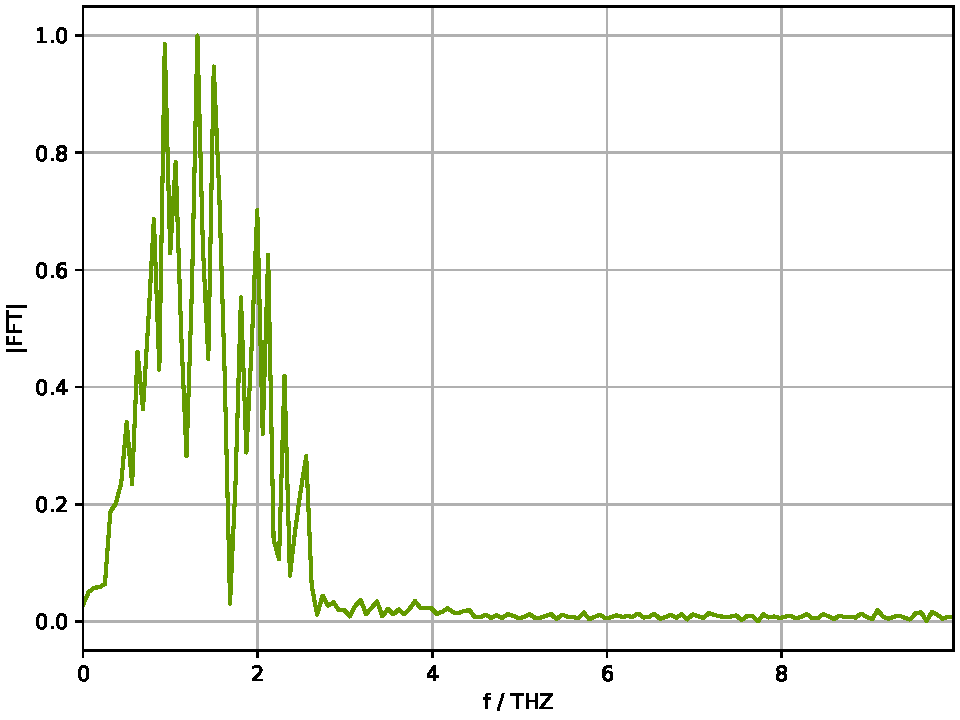
\includegraphics[width=0.8\textwidth]{content/plots/pdf/ZnTe/110mW_fft.pdf}
    \caption{Fourier transform of the THz pulse generated by ZnTe at a pump power of
    $\SI{5}{\milli\watt}$.}
    \label{fig:ZnTeF}
\end{figure}




\section{OH1}
\label{sec:AOH1}
First, the OH1 crystal is tested for the generation of THz radiation.
It should be noted that the crystal, with a size of $\SI{2.24}{\milli\meter\squared}$, fills
only a small part of the pump beam.
which has a beam size of $\SI{67.1+-15.7}{\milli\meter\squared}$, as determined in
\autoref{sec:spot}.
The crystal therefore fills only $3.33\,\%$ of the beam, which reduces the incident
radiation on the crystal by this factor.
In the following, work is first continued with the total pump power, before switching later
to power per unit area for the amplitude comparison with ZnTe.
To begin with, analogous to before in \autoref{sec:AZnTe}, the entire range of the delay
stage is measured in order to find time zero.
The measurement starts at the lowest pump power, which is then increased until a THz pulse
is visible.
This is the case from a pump power of $\SI{7.5}{\milli\watt}$ onward.
The pump power is then continuously increased, and a measurement from
$\SIrange{-2}{6}{\pico\second}$ is performed at each set power.
Since the crystal was not destroyed even at the highest pump power of $\SI{470}{\milli\watt}$,
the sample is moved closer to the focal point in order to increase the power per unit area.
Initially, the crystal was at a distance of $\SI{4.5}{\centi\meter}$ from the lens in front
of the crystal, which has a focal length of $\SI{10}{\centi\meter}$.
The crystal is now moved to a distance of $\SI{7}{\centi\meter}$.
Assuming that the beam is point-like at the focal point, this gives a beam size of
$\SI{20+-4.7}{\milli\meter\squared}$ at the new position.
Here, the ratio of beam to crystal has grown from $3.33\,\%$ to $11.2\,\%$.
In order to obtain an accurate transient at this high power, an interval of
$\SIrange{-6}{11}{\pico\second}$ was measured at this power.
The resulting transient is shown in \autoref{fig:OH1T}.
\begin{figure}
    \centering
    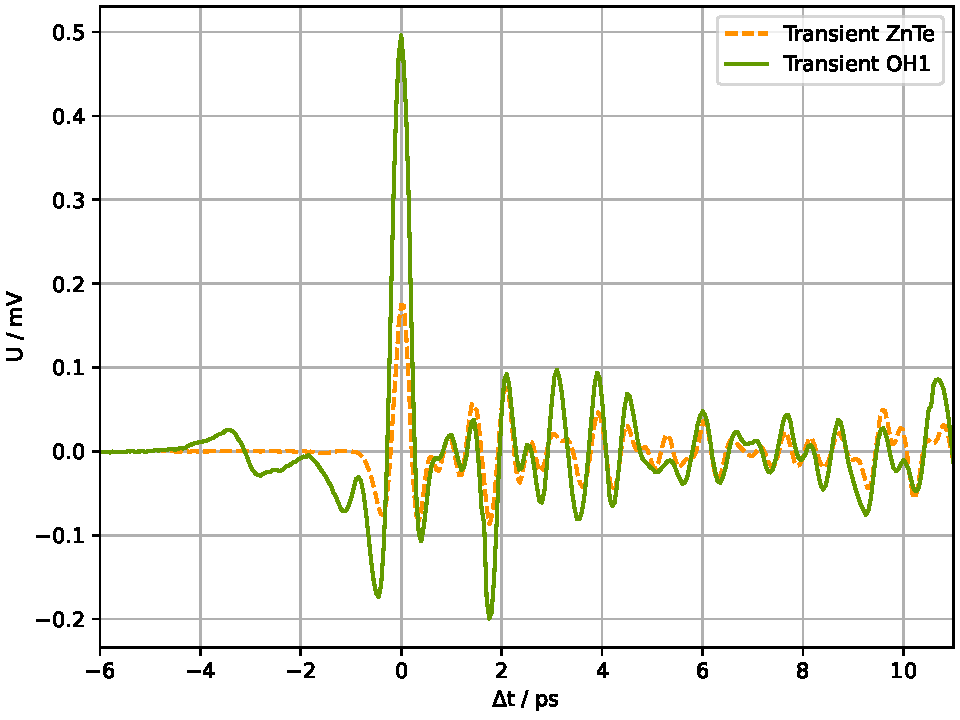
\includegraphics[width=0.8\textwidth]{content/plots/pdf/OH1/470mW,naha,am,fokuspunkt,lange,Messung.pdf}
    \caption{Transient of the THz pulse at a pump power of $\SI{470}{\milli\watt}$.
    With the calculated effective power hitting the crystal of $\SI{52.64}{\milli\watt}$.}
    \label{fig:OH1T}
\end{figure}

In this, time zero can be seen very clearly, with small pre-oscillations that arise because
the pulse starts at low intensity and the actual peak of the THz pulse is only reached at
time zero.
Ringing also occurs after time zero, arising on the one hand from the natural width of the
THz pulse and on the other hand from back-reflections in the crystal and from the pulse
spreading out due to different refractive indices of the air and thus also different flight
durations of the beam.


% Reference circle: center=(76,72) radius=61px
% Hole area: 11681 px
% Crystal area: 5336 px
% Area fraction crystal/hole: 45.7 %
% Scale: 0.0205 mm/px
% Absolute crystal area: 2.241 mm^2
% Control image saved: mask_vis.jpg

\begin{figure}
    \centering
    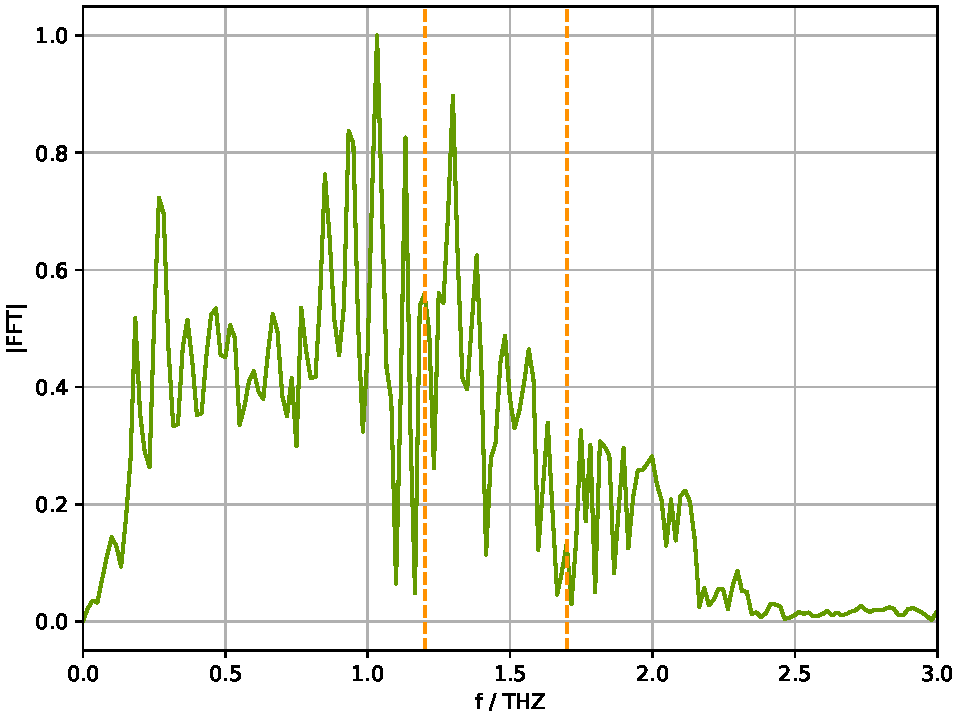
\includegraphics[width=0.8\textwidth]{content/plots/pdf/OH1/470mW,naha,am,fokuspunkt,lange,Messung_fft.pdf}
    \caption{Fourier transform of the THz pulse at a pump power of $\SI{470}{\milli\watt}$.
    With the calculated effective power hitting the crystal of $\SI{52.64}{\milli\watt}$.}
    \label{fig:OH1f}
\end{figure}

Furthermore, \autoref{fig:OH1f} shows the Fourier transform of the transient.
In this, it can be seen that the THz pulse contains frequencies from $\SIrange{0.2}{2.2}{THz}$,
giving a bandwidth of $\SI{2}{THz}$.
In addition, the absorption lines of water at $\SI{1.2}{THz}$ and $\SI{1.7}{THz}$ can also be
seen here.
The peak-to-peak value and the signal-to-noise ratio are then determined for the various
pump powers; these are listed in \autoref{tab:SNOH1}.

\begin{table}
    \centering
    \caption{Peak-to-peak amplitude and the resulting signal-to-noise ratio of the OH1
    transients at various pump powers (selection), relative to the uniform noise reference
    $U_\text{Rausch}=\SI{0.158}{\micro\volt}$ at $\tau=\SI{450}{ms}$.}
    \label{tab:SNOH1}
    \begin{tabular}{l S[table-format=3.1] S[table-format=4.1]}
        \toprule
        {$P \mathrel{/} \si{\milli\watt}$} & {$U_\text{ptp} \mathrel{/} \si{\micro\volt}$} & {SNR} \\
        \midrule
        8                        & 15.4  & 97.3   \\
        17.3                     & 7.2   & 45.5   \\
        24.2                     & 11.2  & 70.9   \\
        30                       & 77.5  & 490.7  \\
        38                       & 20.2  & 127.9  \\
        74                       & 56.4  & 357.2  \\
        270                      & 88.5  & 559.8  \\
        350                      & 108.8 & 688.8  \\
        470                      & 139.2 & 880.8  \\
        \bottomrule
    \end{tabular}
\end{table}


The peak-to-peak values are also compared with those of the ZnTe crystal in \autoref{fig:ampc}.
Here, however, the pump power is no longer used for the OH1 crystal; instead, the power per
unit area multiplied by the area of the crystal is used.
The power density was determined in \autoref{sec:spot} to be
$\SI{0.103+-0.024}{\watt\per\centi\meter\squared}$, and the area of the crystal was
determined using photos and a Python script to be $\SI{2.241}{\milli\meter\squared}$.
Using these values, \autoref{fig:ampc} is obtained.


\begin{figure}
    \centering
    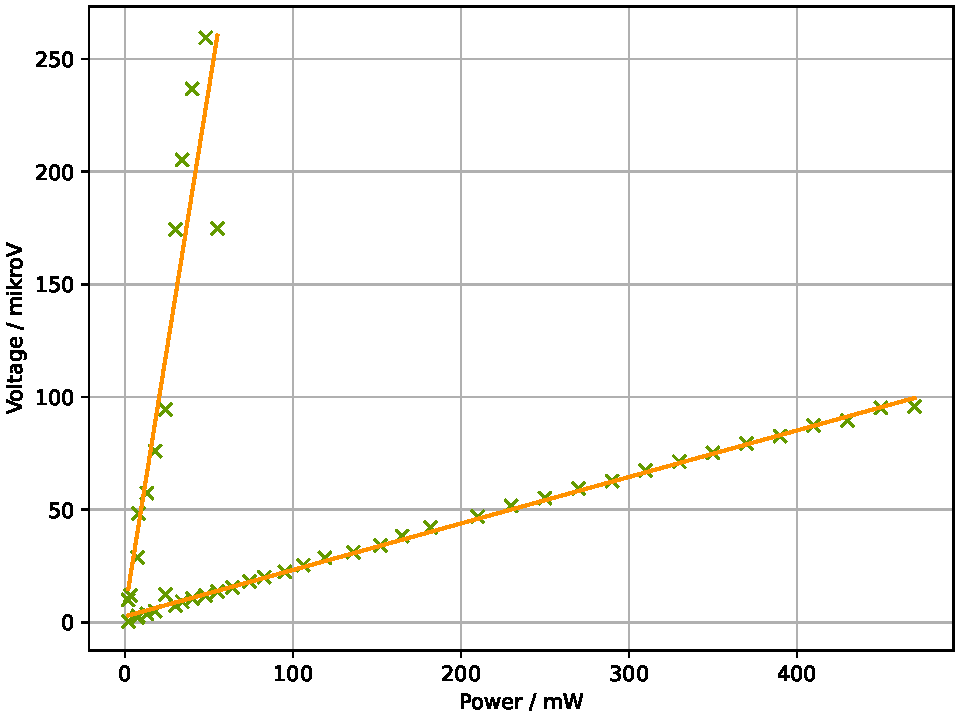
\includegraphics[width=0.8\textwidth]{content/plots/pdf/amplitude_comb.pdf}
    \caption{Comparison of the amplitude of THz pulses from ZnTe and OH1.
    For comparison, a linear fit was applied through both data series.}
    \label{fig:ampc}
\end{figure}

Since the crystal has a significantly smaller area than the ZnTe crystal and therefore also
absorbs less power, this is reflected in \autoref{fig:ampc}, in that the OH1 values, in
contrast to ZnTe, all lie at low powers.
Furthermore, it is found that the amplitude of the THz radiation generated by OH1 rises
somewhat less steeply than that of ZnTe.
The deviating measured values between $\SIrange{30}{48}{\milli\watt}$ mentioned in
\autoref{sec:AZnTe} can also be seen in the plotted values of the ZnTe crystal.

\section{BNA}
\label{sec:ABNA}

For BNA, as with the other materials before, a large range was scanned and the pump power
was then progressively increased from $\SIrange{2.2}{480}{\milli\watt}$.
The transient for the highest pump power is shown in \autoref{fig:BNAt}.
It can be seen there that no peak is visible and only noise was measured.
This initially suggests that no significant THz radiation could be generated with the
sample used.
The reasons for this are explained in the following.

\begin{figure}
    \centering
    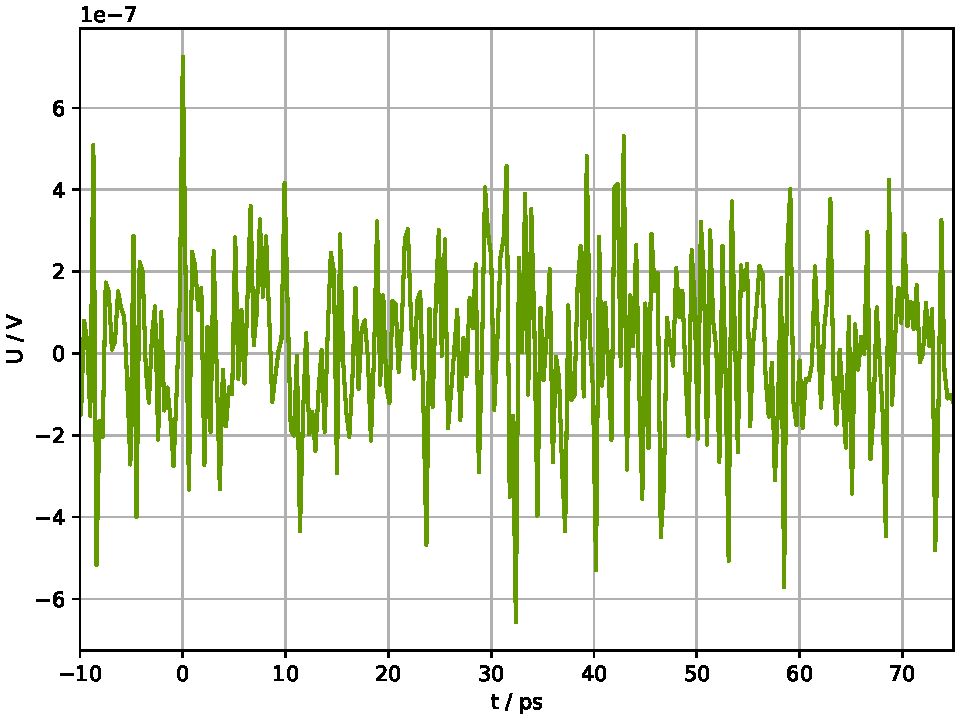
\includegraphics[width=0.8\textwidth]{content/plots/pdf/BNA/480mW,real.pdf}
    \caption{Transient of the THz pulse at a pump power of $\SI{480}{\milli\watt}$.
    No signal above the noise level can be discerned.}
    \label{fig:BNAt}
\end{figure}

The samples were very small, powder-like crystals, and for individual crystallites it could
not be reliably determined whether they were actually single crystals; their diameter was at
most $\SI{2}{\milli\meter}$.
The sample used was examined under a microscope for irregularities and other anomalies.
\autoref{fig:my8} shows an eightfold magnification of the sample.
Irregularities and various layers can be seen in it.
One of these irregularities is marked, having a length of $\SI{0.228}{\milli\meter}$.
As a result, if many different crystals are present in the sample, they also always have
different orientations.
Due to this orientation, the individual crystals each generate THz radiation on their own,
but this radiation has, in each case, a different polarization direction and phase relative
to one another.
As a result, in the extreme case, the generated THz field averages out to zero over a very
large number of small crystals.
In addition, this sample is also very small, with an area of $\SI{6.28}{\milli\meter\squared}$.
The effective power hitting the crystal is therefore a factor of 3 larger than for OH1, but
still one tenth smaller than for ZnTe.
Thus, due to the quality of the sample, no statement can be made about the material's
usability for generating THz radiation.



%5.632/2560=0.0022mm/pixel
%8x magnification, i.e. 0.000275 mm/pixel
%574*599=829.62 pixels
%Length = 0.228mm


\begin{figure}
    \centering
    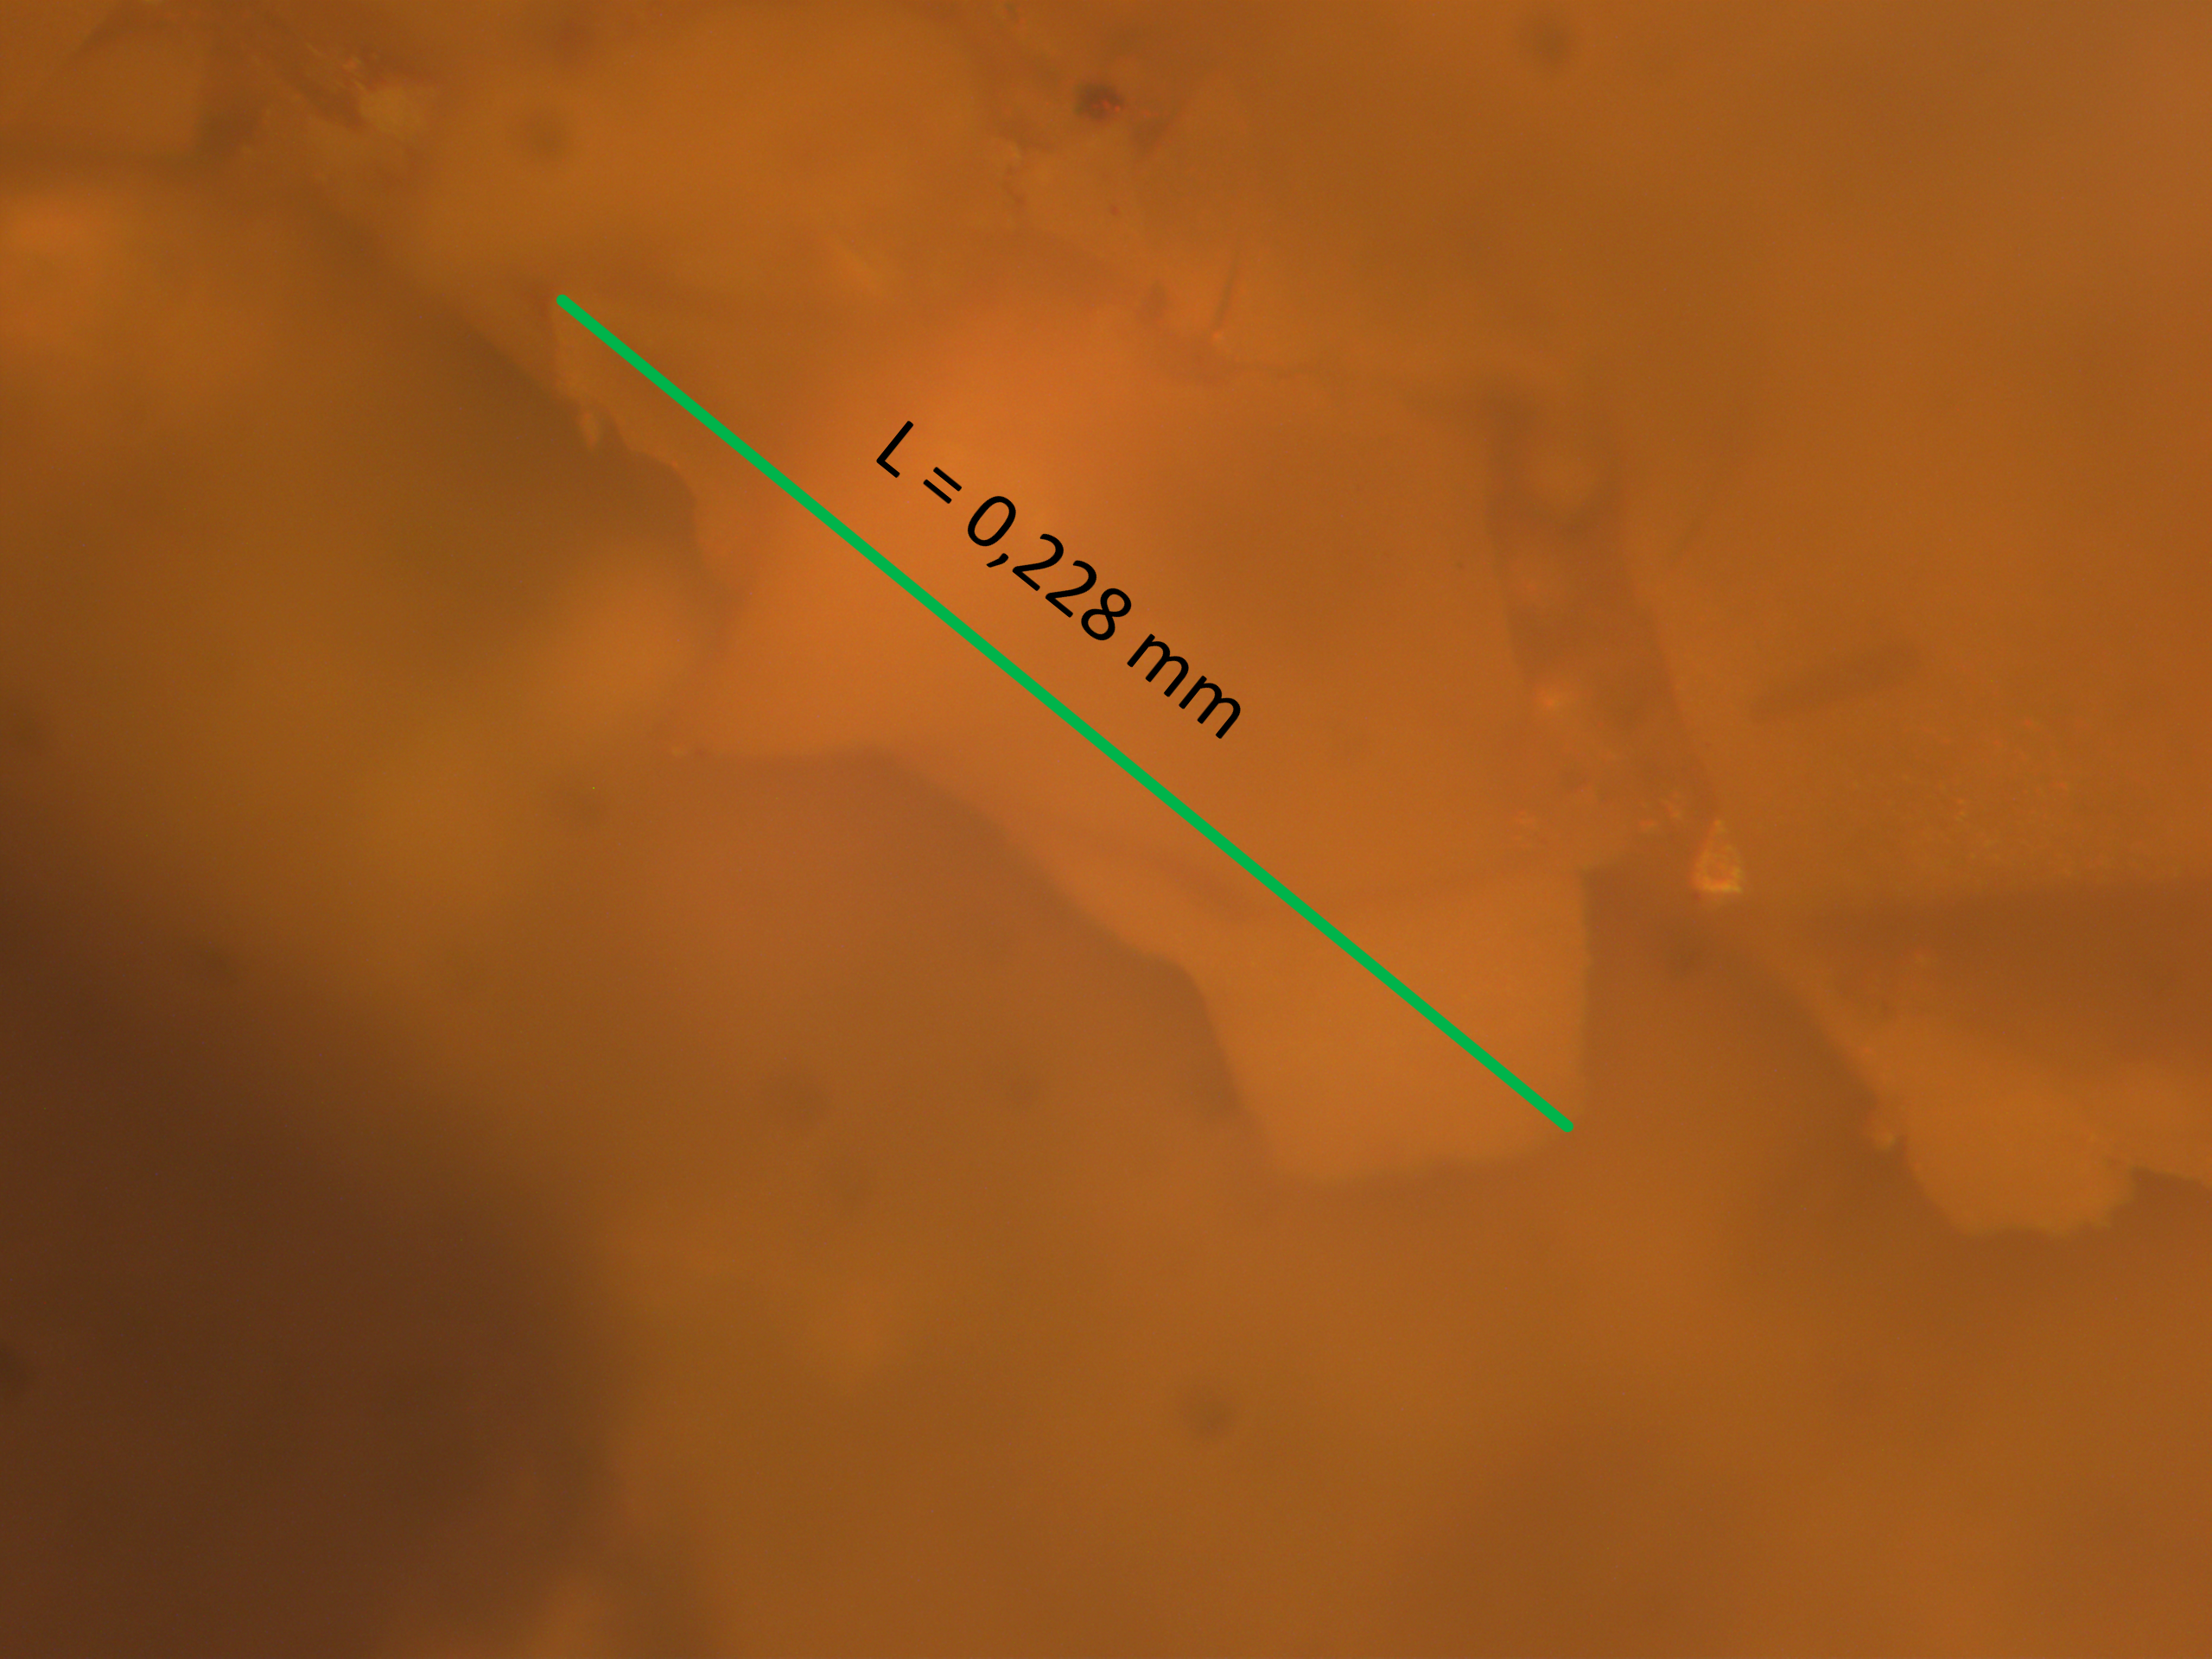
\includegraphics[width=0.8\textwidth]{content/bilder/mikroskop/yellow_drauflicht_8x.png}
    \caption{Eightfold magnification of the BNA sample used, with a marked irregularity of
    length $L=\SI{0.228}{mm}$.}
    \label{fig:my8}
\end{figure}


% \begin{figure}
%     \centering
%     \includegraphics[width=0.8\textwidth]{content/plots/build/OH1/transients/202608071724_1Dx1D_756ed8_470mW_naha_am_fokuspunkt_lange_Messung.pdf}
%     \caption{Comparison of the noise voltage with and without the laser switched on.}
%     \label{fig:tcc}
% \end{figure}
% \begin{figure}
%     \centering
%     \includegraphics[width=0.8\textwidth]{content/plots/build/OH1/transients/202608071709_1Dx1D_40e4a3_470mW_naeher_am_Fokus2.pdf}
%     \caption{Comparison of the noise voltage with and without the laser switched on.}
%     \label{fig:tcc}
% \end{figure}

% \begin{figure}
%     \centering
%     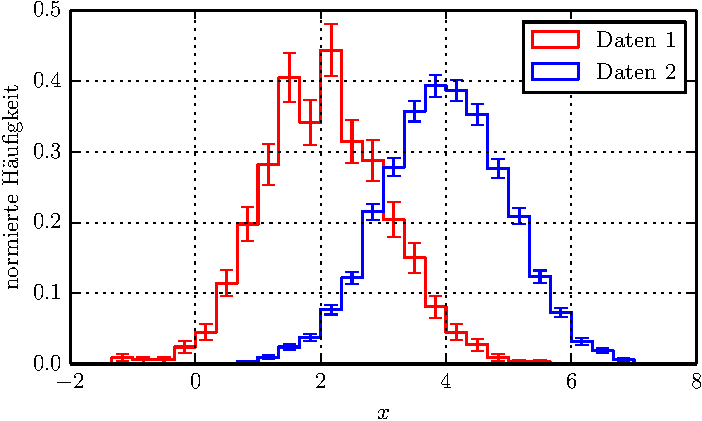
\includegraphics[\textwidth]{./Plots/Histogramm.pdf}
%     \caption{A histogram with error bars for two data sets; the font size and typeface match
%     those of the document.}
%     \label{fig:bsp}
% \end{figure}

